\chapter{Disertantes}

Presentamos aqu� los disertantes de cada evento con una breve biograf�a y sus campos de investigaci�n.

\section*{Encuentro de Estudiantes de �ptica y Fotof�sica (EEOF)}

%%%%%%%%%%%%%%%%%%% STEFANI
\subsection*{Fernando Stefani}

\begin{wrapfigure}{l}{0.09\textwidth}
\vspace{-20pt}
  \begin{center}
  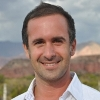
\includegraphics[width=0.08\textwidth]{fstefani}
  \end{center}
\label{fg:fstefani}
\vspace{-30pt}
%\caption{rmenon}
%\vspace{-10pt}
\end{wrapfigure}

Nanophysics Group Lab\\
Phisics Department, FCEyN, UBA. Argentina. fernando.stefani@df.uba.ar \\

\subsubsection*{Research fields}

\begin{itemize}
\item    Metallic, semiconducting and magnetic nanoparticles
\item    Organic fluorophores
\item    Conjugated polymers
\item    Supramolecular structures
\item    Hybrid nanobiosystems
\item    Proteins and DNA

\end{itemize}

\subsubsection*{Short biography}
\begin{itemize}    
\item   born 19.11.1975 in Buenos Aires
\item   Materials Engineering studies at the Instituto de Tecnolog�a Prof. Jorge Sabato (IT) - Buenos Aires, Argentina
\item   2004 PhD at the Max-Planck-Institute for Polymer Research (MPIP, Prof. Dr. W. Knoll) - Mainz, Germany
\item   2004-2006 Postdoc at the MPIP (Prof. Dr. W. Knoll) - Mainz, Germany
\item   2006-2008 Research fellow at the Institute of Photonic Sciences (ICFO, Prof. Dr. Niek van Hulst) - Barcelona, Spain
\item   2008-2009 Group leader the Physics Department of the Ludwig-Maximilians-Universit�t M�nchen (LMU, Prof. Dr. Jochen Feldmann) - Munich, Germany
\item   Since 2009 Associate Researcher of the National Research Council (CONICET) and head of the Applied nanoPhysics Group at the Physics Department of the University of  Buenos Aires (UBA) - Buenos Aires, Argentina
\item   Since 2010 Associate Professor of the Physics Department of the University of Buenos Aires (UBA), Buenos Aires, Argentina.
\item   Since 2011 leader of a Max-Planck-Society Partner Group in collaboration with the Nanobiophotonics group of Prof. Stefan W. Hell at the MPI biophysikalische Chemie (G�ttingen).
\end{itemize}


%%%%%%%%%%%%%%%%%%%%%%%%% BRAGAS
\subsection*{Andrea Bragas}

\begin{wrapfigure}{l}{0.09\textwidth}
\vspace{-20pt}
  \begin{center}
  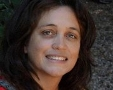
\includegraphics[width=0.08\textwidth]{abragas}
  \end{center}
\label{fg:abragas}
\vspace{-30pt}
%\caption{rmenon}
%\vspace{-10pt}
\end{wrapfigure}

Quantum electronics Laboratory. \\
Phisics Department, FCEyN, UBA. Argentina. bragas@df.uba.ar \\

\subsubsection*{Research fields}

\begin{itemize}
\item   High resolution optical microscopy
\item   Plasmonic probes
\item   Vibrations of plasmonic objects and ensembles
\item   Linear and nonlinear optical properties of nanomaterials.
\end{itemize}

\subsubsection*{Short biography}
    
Andrea Bragas is one of the heads of the Quantum Electronics Lab at the University of Buenos Aires and professor at the School of Sciences. Her current research fields are focused on the fabrication, study and control of different isolated and interacting plasmonic objects with the aim of their application to high-resolution microscopies, chemical and biological sensing, bio-imaging, and development of nano-light sources. \\


%%%%%%%%%%%%%%%%%%%%%%%%%%%% MAIER
\subsection*{Stefan Maier}

\begin{wrapfigure}{l}{0.09\textwidth}
\vspace{-20pt}
  \begin{center}
  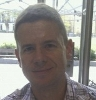
\includegraphics[width=0.08\textwidth]{smaier}
  \end{center}
\label{fg:smaier}
\vspace{-30pt}
%\caption{rmenon}
%\vspace{-10pt}
\end{wrapfigure}

Nanoplasmonics group. \\
Imperial College, London, UK. s.maier@imperial.ac.uk \\

\subsubsection*{Research fields}

\begin{itemize}
\item    Nanocavities: Fundamentals and applications in energy concentration and biosensing 
\item    Optical and THz Metamaterials 
\item    Nanoantennas and enhanced Light/Matter coupling 
\item    Active Plasmonics and Plasmon Waveguides
\end{itemize}

\subsubsection*{Short biography}
    
Stefan Maier is Professor of Nanophotonics in the Department of Physics at Imperial College London, and co-director of the College's Centre for Plasmonics and Metamaterials. He obtained his PhD in Applied Physics at 2003 at the California Institute of Technology. Stefan has published over 130 papers in plasmonics and nanophotonics, is a fellow of OSA, and was awarded the Sackler Prize in the Physical Sciences and the Paterson Medal of the Institute of Physics. He further holds a Royal Society Wolfson Research Merit Award.\\


%%%%%%%%%%%%%%%%%%%%%%%%%% MENON
\subsection*{Rajesh Menon}

\begin{wrapfigure}{l}{0.09\textwidth}
\vspace{-20pt}
  \begin{center}
  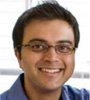
\includegraphics[width=0.08\textwidth]{rmenon}
  \end{center}

\label{fg:rmenon}
\vspace{-30pt}
%\caption{rmenon}
%\vspace{-10pt}
\end{wrapfigure}

Laboratory for Optical Nanotechnologies. \\
University of Utah, Utah, USA. rmenon@eng.utah.edu \\

\subsubsection{Short biography}

Rajesh Menon has pioneered several technologies that will enable far-field optics to manipulate and image matter with nanoscale resolution, something that was thought impossible until a few years ago. His research has spawned over 50 publications, over 30 patents, and 2 spin-off companies. He has led several projects in nanopatterning and nanoscopy with support from DARPA, the NSF, US Air Force, and the MIT Deshpande Center for Technological Innovation. Among his honors are an NSF CAREER Award (2011) and the International Commission for Optics Prize (2009).\\
He currently directs the Laboratory for Optical Nanotechnologies at the University of Utah. Prior to that, Prof. Menon was a research engineer at MIT's Research Laboratory of Electronics, where he remains a research affiliate. He holds S.M. and Ph.D. degrees from the Department of Electrical Engineering and Computer Science at MIT. In addition, he served as the Chief Technology Officer of LumArray, a company he co-founded with colleagues at MIT. \\

\subsubsection{Research fields}
\begin{itemize}
\item Absorbance Modulation Optical Lithography (AMOL) 
\item Patterning via Optical Saturable Transformations (POST) 
\item Ultra-high efficiency photovoltaics via Diffractive Spectrum Separation 
\item Optimized Nanophotonics for efficient ultra-thin-film photovoltaics 
\item 3D tracking of surgical instruments 
\end{itemize}



% y tal vez de que hablaran